

\begin{figure}[h]


    \centering
    
    % \hspace{2em}
    \textbf{MATLAB}\hspace{14em}
    \textbf{Python}
    
    \hspace{-2em}
    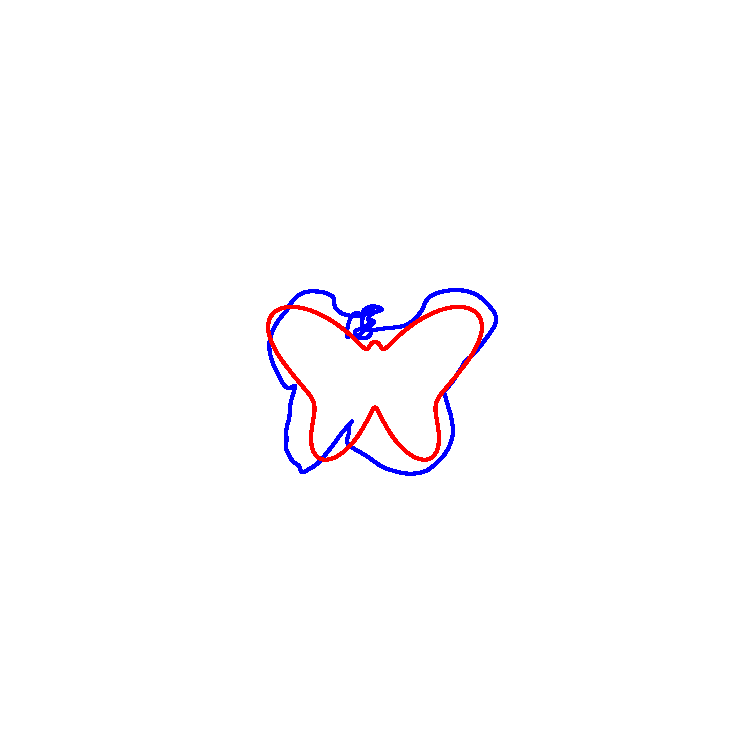
\includegraphics[trim=3cm 4cm 3cm 4cm, clip=true, height=.25\linewidth]{Figures/Fig_T7/MATLAB/RMHL_T1_Trajectory.eps}
    \hspace{4em}
    \includegraphics[trim=6.5cm 4.5cm 6cm 4.5cm, clip=true,  height=.25\linewidth]{Figures/Fig_T7/Python/RMHL_T1_Jmat_Trajectory.eps} \\
    
    
    
    
        \textbf{\rotatebox[origin=c]{90}{x(t)}}\begin{subfigure}{\textwidth}
        \centering
        
        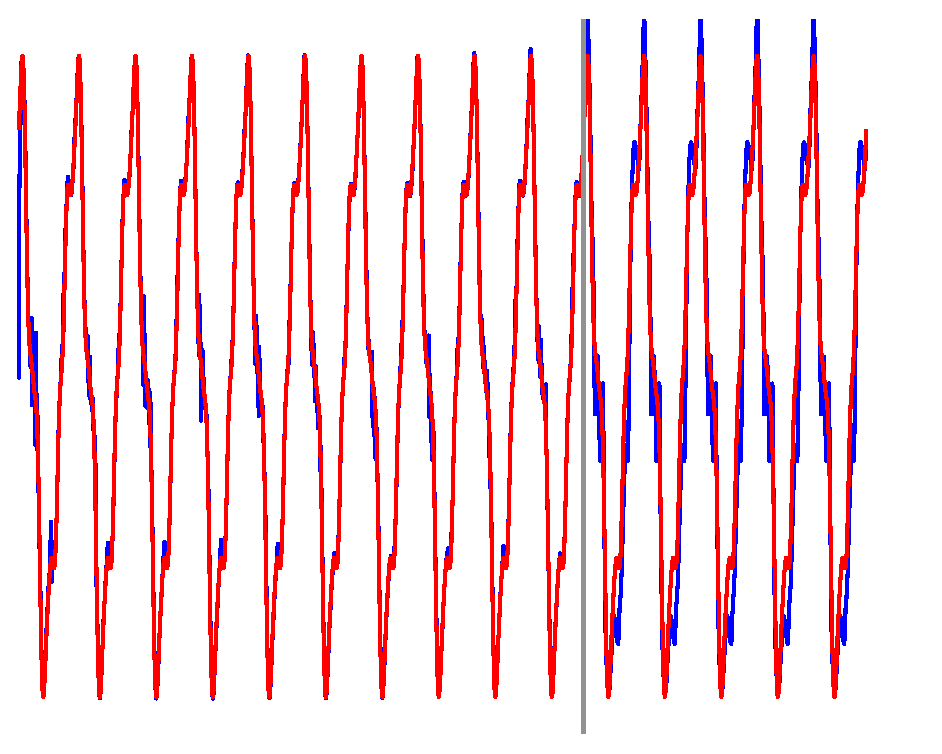
\includegraphics[trim=0cm 0cm 0cm 0cm,clip=true,height=0.1\linewidth,width=.45\linewidth]{Figures/Fig_T7/MATLAB/RMHL_T1_CoordinateX.eps}
        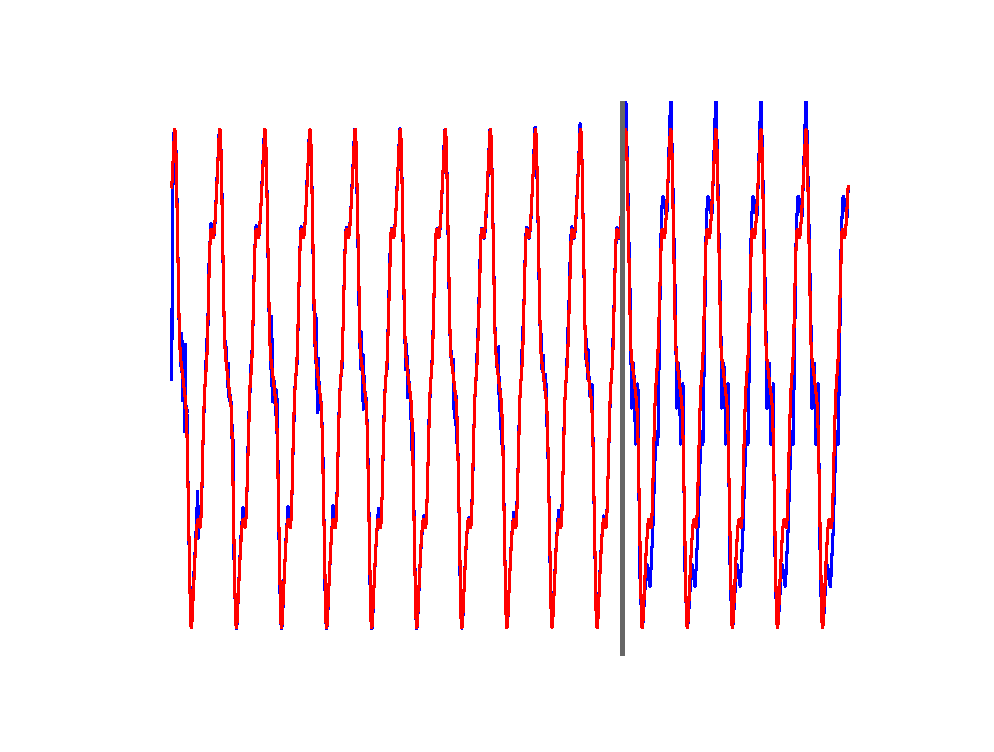
\includegraphics[trim=2cm 1cm 2cm 1cm,clip=true,height=0.1\linewidth,width=.45\linewidth]{Figures/Fig_T7/Python/RMHL_T1_Jmat_CoordinateX.eps}\\
    
    \end{subfigure}
    
    
        \textbf{\rotatebox[origin=c]{90}{y(t)}}\begin{subfigure}{\textwidth}
        \centering
        
        \includegraphics[trim=0cm 0cm 0cm 0cm,clip=true,height=0.1\linewidth,width=.45\linewidth]{Figures/Fig_T7/MATLAB/RMHL_T1_CoordinateY.eps}
        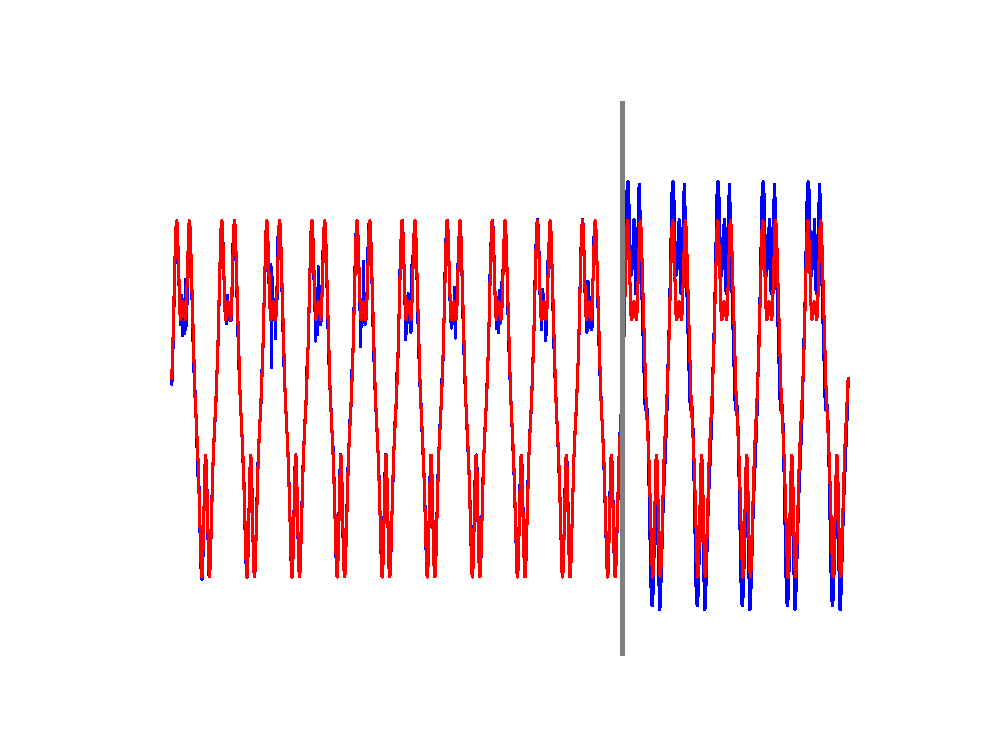
\includegraphics[trim=2cm 1cm 2cm 1cm,clip=true,height=0.1\linewidth,width=.45\linewidth]{Figures/Fig_T7/Python/RMHL_T1_Jmat_CoordinateY.eps}   
    
    \end{subfigure}
    
    
    \vspace{4em}
    
    \textbf{\rotatebox{90}{$||W||$}}\begin{subfigure}{\textwidth}
        \centering
        
        \hspace{.5em}
        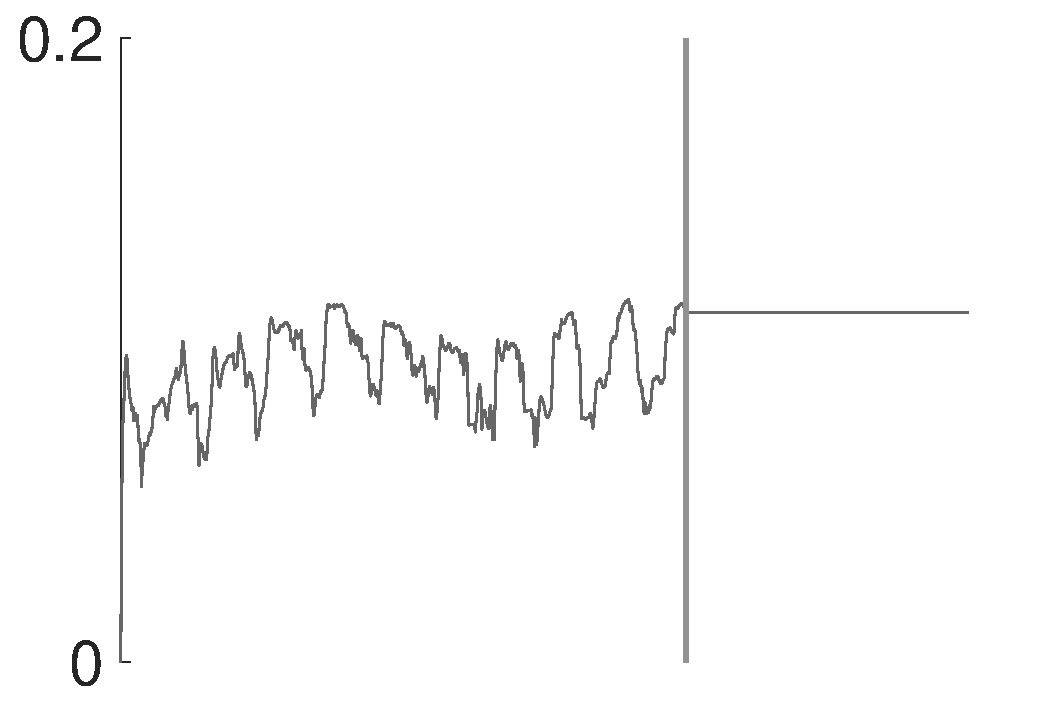
\includegraphics[trim=0cm 0cm 0cm 0cm,clip=true,height=0.15\linewidth,width=.45\linewidth]{Figures/Fig_T7/MATLAB/RMHL_T1_W_norm.eps}
        \hspace{0em}
        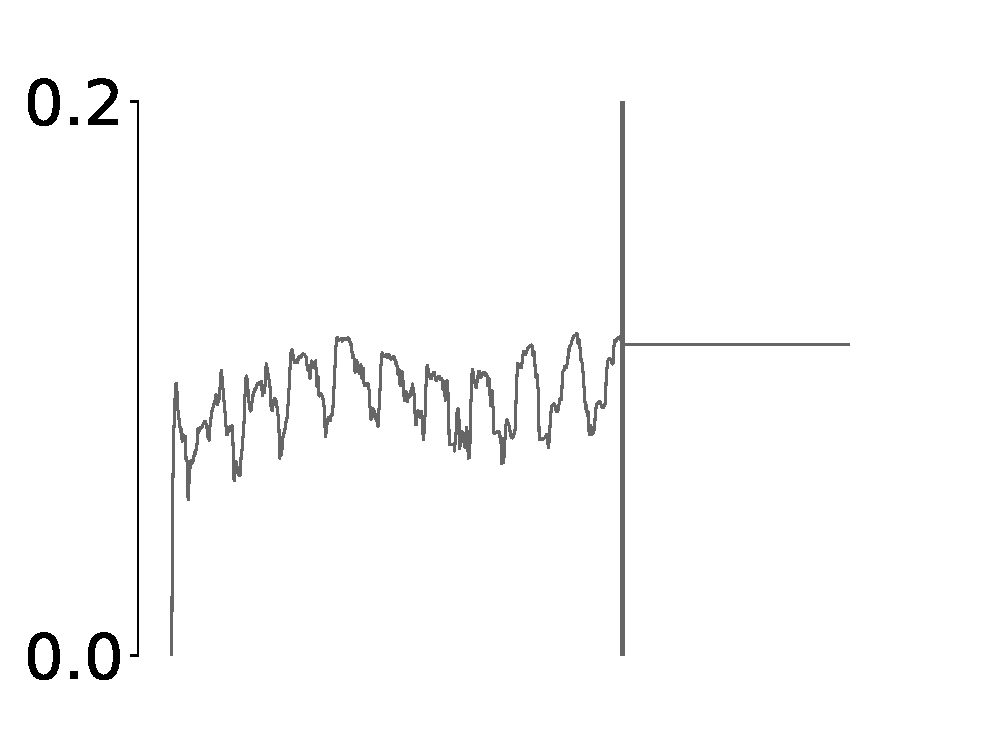
\includegraphics[trim=0cm 0.5cm 2cm 0.5cm,clip=true,height=0.15\linewidth,width=.45\linewidth]{Figures/Fig_T7/Python/RMHL_T1_Jmat_W_norm.eps}
    
    \end{subfigure}
    
    
    \vspace{2em}
    
    \textbf{\rotatebox{90}{MSE}}\begin{subfigure}{\textwidth}
        \centering
        
        \hspace{.5em}
        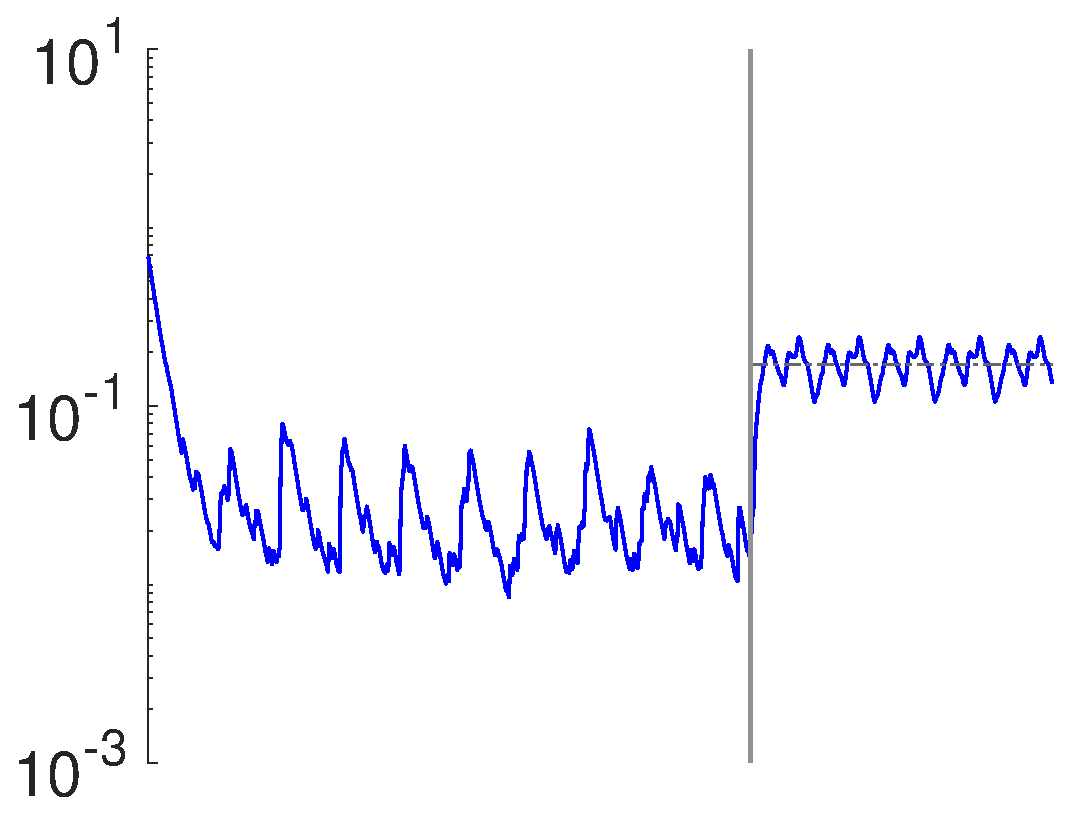
\includegraphics[trim=0cm 0cm 0cm 0cm,clip=true,height=0.15\linewidth,width=.45\linewidth]{Figures/Fig_T7/MATLAB/RHML_T1_Jmat_MSE.eps}
        \hspace{1em}
        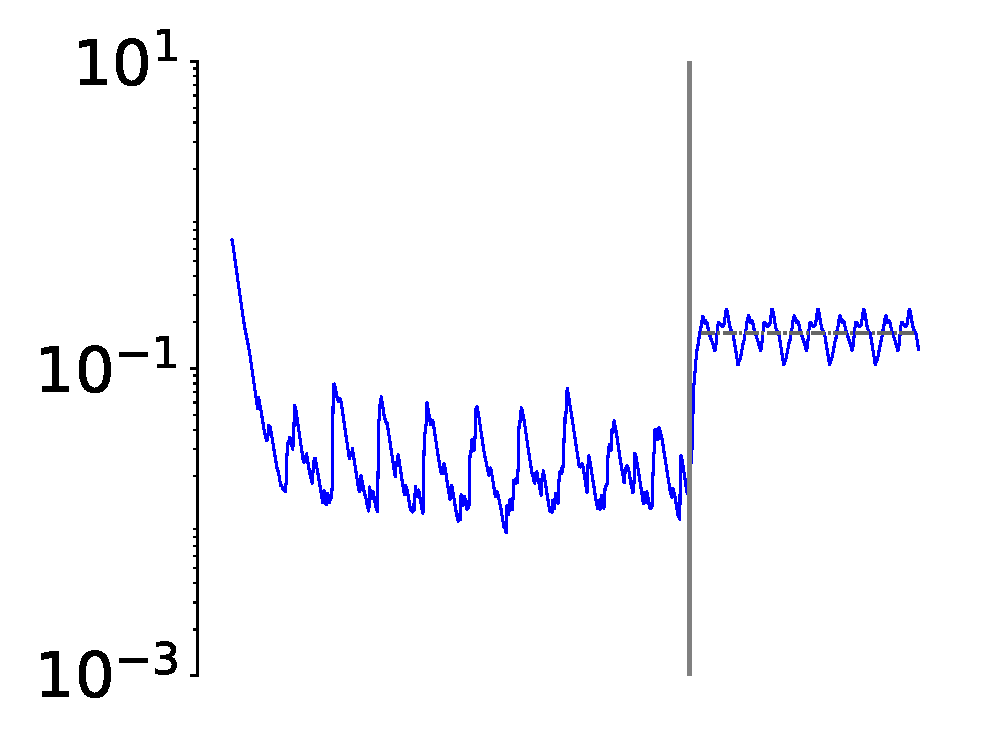
\includegraphics[trim=0cm 0cm 0cm 0cm,clip=true,clip=true,height=0.15\linewidth,width=.45\linewidth]{Figures/Fig_T7/Python/RMHL_T1_Jmat_MSE.eps}
    
    \end{subfigure}
        
            

        
    
        
        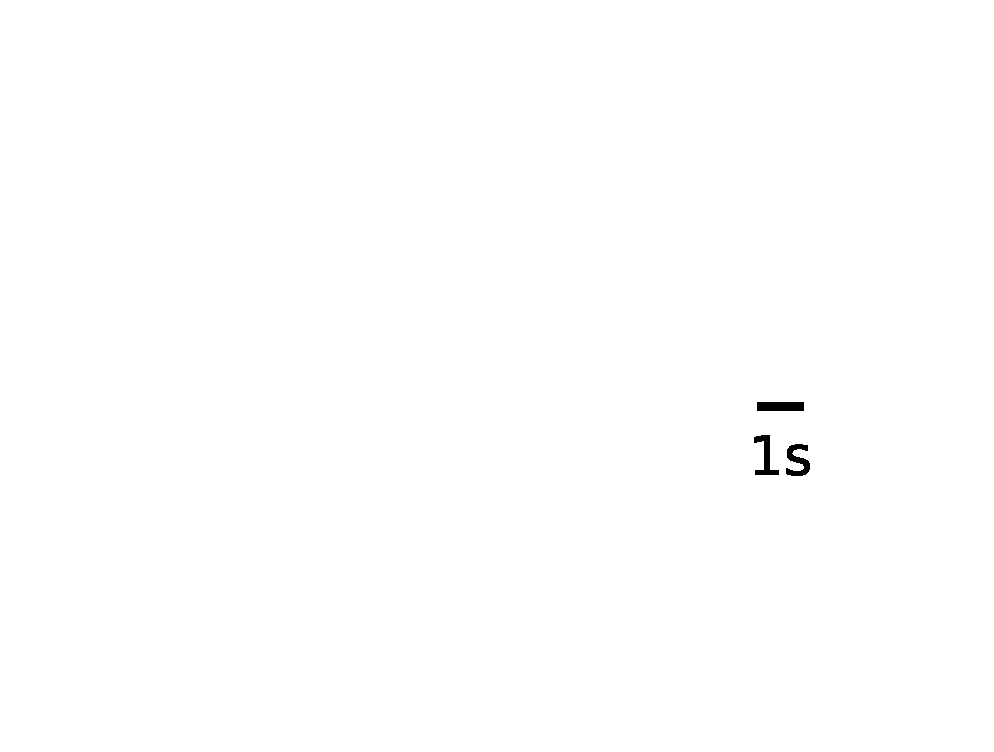
\includegraphics[trim=2cm 6cm 2cm 6cm, clip=true,height=0.05\linewidth,width=.4\linewidth]{Figures/Fig_T1/Python/ST_T1_Scale.eps}
        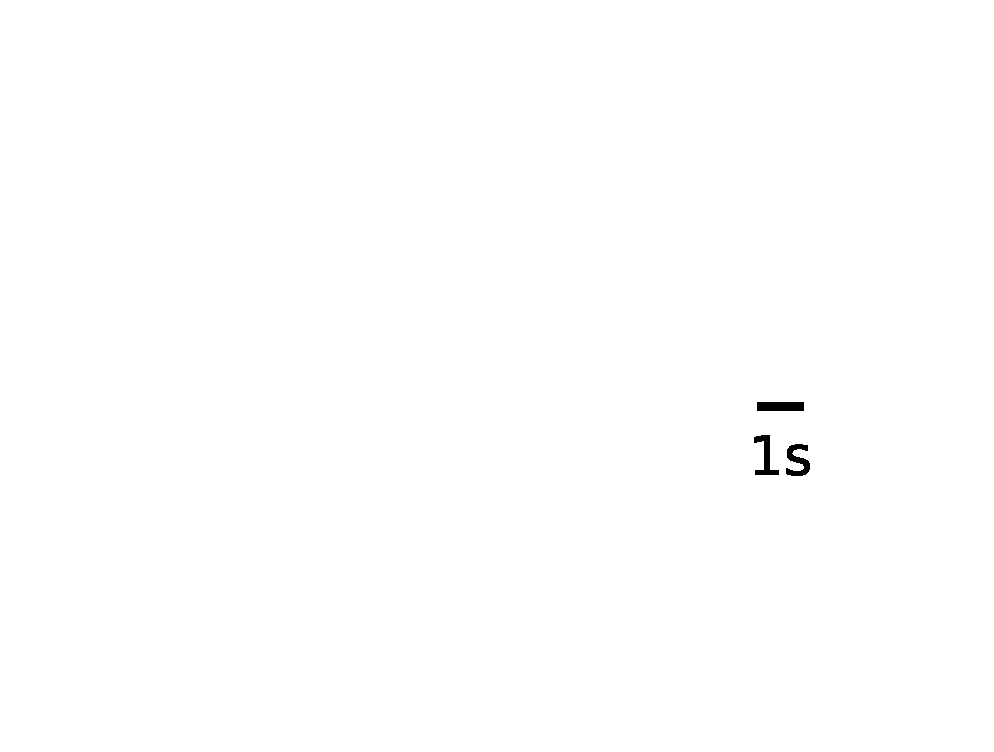
\includegraphics[trim=2cm 4cm 2cm 6cm, clip=true,height=0.05\linewidth,width=.45\linewidth]{Figures/Fig_T1/Python/ST_T1_Scale.eps}


\caption{Similarity between the original scripts and the Python adaptation. The performance of the original scripts (left column) and the Python adaptation (right column) is tested for the RMHL learning algorithm on a Task 1. The reservoir connectivity matrix for the Python simulation was initialised using the MATLAB equivalent. Using this initialisation, the progression of the Python simulation is identical to that of the MATLAB simulation. The top panel shows the target trajectory (red) with the trajectory generated by the model (blue) throughout the test phase. The next two rows show the time-series (blue) generated by the model (x and y coordinates, in this case). The third row shows the progression of the norm of the weight matrix. The bottom row shows the distance from target metric (blue) over the simulation, using the log scale for the y axis. The horizontal grey line, in the test phase, indicates the deviation metric. The grey vertical line marks the separation of the training and testing phase.}
\label{Fig:Comparison_sprandn}

\end{figure}